\documentclass[bachelor, och, coursework]{SCWorks}
\usepackage[T2A]{fontenc}
\usepackage[cp1251]{inputenc}
\usepackage{graphicx}
\usepackage[sort,compress]{cite}
\usepackage{amsmath}
\usepackage{amssymb}
\usepackage{amsthm}
\usepackage{fancyvrb}
\usepackage{longtable}
\usepackage{array}
\usepackage[english,russian]{babel}
\usepackage{tempora}
\usepackage{minted}

\usepackage[colorlinks=true]{hyperref}


\newcommand{\eqdef}{\stackrel {\rm def}{=}}

\newtheorem{lem}{?????}
\begin{document}
\chair{математической кибернетики и компьютерных наук}
\title{Правила оформления курсовых и дипломных работ}
\course{1}
\group{111}
\napravlenie{02.03.02 "--- Фундаментальная информатика и информационные технологии}
\author{Дербина Даниила Михайловича}
\chtitle{к.\,ф.-м.\,н.} 
\chname{С.\,В.\,Миронов}
\satitle{доцент, к.\,ф.-м.\,н.} 
\saname{А.\,С.\,Иванова}
\patitle{к.\,ф.-м.\,н., доцент}
\paname{Д.\,Ю.\,Петров}
\term{2}
\practtype{учебная}
\duration{3}
\practStart{26.04.2022}
\practFinish{16.05.2022}
\date{2022}
\maketitle
\tableofcontents
\abbreviations
\begin{description}
    \item[ДКА] "--- детерменированный конечный автомат.
    \item[КС-грамматика] "--- контекстно-свободная грамматика.
    \item[ПС-анализатор] "--- анализатор типа <<перенос-свертка>>.
    \item[ДКАПС-анализ] "--- анализ типа <<перенос-свертка>>.
    \item[ДКААСД] "--- абстрактное синтаксическое дерево.
\end{description}
\intro
Лексические и синтаксические анализаторы как предмет научного 
исследования появились в 1950"=х годах XX века. 
Бурный рост интереса был обусловлен в том числе необходимостью 
создания интерпретаторов и компиляторов для
трансляции языков высокого уровня в другие языки 
или напрямую в машинный код.

Несмотря на то, что сейчас эта область является хорошо изученной, 
она все еще актуальна и находит свои применения при создании 
статических и динамических компиляторов, трансляции одних 
языков программирования в другие, обработке SQL"=запросов 
и некоторых других классов задач [1,2]. Необходимость 
быстрого анализа при этом очевидна.

Целью данной работы является изучение работы лексических 
и синтаксических анализаторов и повышение эффективности анализа 
за счет различных оптимизаций работы с оперативной памятью.

В ходе написания работы должны быть решены следующие задачи:
\begin{enumerate}
    \item Изучение понятий лексического и синтаксического анализа.
    \item Анализ технических особенностей реализации лексических 
    и синтаксических анализаторов и изучение работы генераторов 
    лексического и синтаксического анализа на примере Flex и GNU Bison.
    \item Создание лексического и синтаксического анализатора для 
    анализа математического выражения.
    \item Изучение понятия абстрактного синтаксического дерева.
    \item Создание нескольких реализаций абстрактного 
    синтаксического дерева для построенной грамматики 
    и сравнение эффективности их работы.
\end{enumerate}

\section*{Анализ выражений}
\addcontentsline{toc}{section}{Анализ выражений}

\section{Абстрактные синтаксические деревья}
\subsection{Управление памятью на основе регионов}
\subsubsection{Мотивировка}

Текущая реализация абстрактного синтаксического дерева имеет 
следующие недостатки:

\begin{enumerate}
    \item Выделение памяти стандартным методом может значительно 
    фрагментировать оперативную память, затрудняя доступ к ней.
    \item Любое выделение и удаление памяти требует вмешательства 
    системных вызовов, что может стать причиной дополнительных 
    издержек во время работы программы.
    \item Программист не имеет возможности ручного управления 
    выделяемой им памятью.
\end{enumerate}

Избавиться от этих недостатков можно используя различные оптимизации. 
В рамках этой работы воспользуемся управлением памятью на основе, так
называемых, регионов (арен, зон) ~\cite{D_C_A_Wang_Princeton_University_2002}.

Под регионом далее будем понимать непрерывную область памяти, 
содержащую внутри себя объекты. При запуске программы выделим 
регион некоторого размера, при необходимости увеличивая его 
размер в некоторое постоянное число раз.

Этот подход имеет следующие преимущества:


\begin{enumerate}
    \item Элементы располагаются последовательно, в связи 
    с чем минимизируется фрагментация и упрощается доступ к 
    объектам.
    \item Выделение и освобождение памяти выполняется с 
    минимальными издержками.
    \item Программисту предоставляется большая свобода для 
    управления выделенной памятью.
\end{enumerate}

\subsubsection{Построение}

Формально определим требования к системе:

\begin{enumerate}
    \item Регион должен представлять из себя некоторый 
    непрерывный участок размера $n$ байт (в начальный 
    момент времени размер равен некоторой начальной величине 
    $n_0$).
    \item При обращении к региону он должен предоставить $k$ 
    байт памяти и вернуть некоторый идентификатор этого 
    участка для последующего обращения.
    \item При заполнении региона должна быть возможность 
    увеличить объем доступной памяти в некоторое число раз, 
    которое далее будем называть коэффициентом увеличения.
    \item Должна быть доступна возможность эффективного 
    освобождения всей выделенной регионом памяти.
\end{enumerate}

Единственной сложной операцией над регионом является его 
увеличение. Так как выделение нового участка потенциально 
может сопровождаться изменением адресов объектов, то 
необходимо организовать доступ к ним независимо от первоначального 
адреса. Для этого для каждого объекта будем получать
доступ к нему через некоторый индекс.

Кроме того, коэффициент увеличения должен быть выбран таким 
образом, чтобы был соблюден баланс между оптимальным объемом 
выделенной памяти и частотой системных вызовов.


\subsubsection{Определение структуры}

\setminted{
	style=bw,
	framesep=2mm, 
	baselinestretch=1.2, 
	fontsize=\small, 
	linenos,
	breaklines=true
}

Определим нашу структуру следующим образом:

\begin{minted}{cpp}
typedef struct arena {
	// Указатель на начало региона
	struct node* arena;
	// Размер региона
	unsigned int size;
	// Объем выделенной регионом памяти
	unsigned int allocated;
} arena;
\end{minted}

\subsubsection{Инициализация}

Теперь определим функцию \verb"arena_construct", выполняющую начальную
инициализацию состояния региона:

\begin{minted}{cpp}
int arena_construct (arena* arena) {
	// Начальный размер региона равен некоторой постоянной, равной DEFAULT_ARENA_SIZE
	arena->size = DEFAULT_ARENA_SIZE;
	arena->allocated = 0;
	// Выделим необходимое число памяти
	arena->arena = malloc(sizeof(node) * DEFAULT_ARENA_SIZE);
	// Если выделение прошло неудачно - вернем в качестве кода ошибки отличное от 0 значение.
	if (arena->arena == NULL) {
		return (!0);
	}
	return 0;
}
\end{minted}


\subsubsection{Выделение памяти}

После выделения некоторого объема памяти возможно обращение к ней.
Определим это обращение с помощью функции \verb"arena_allocate":

\begin{minted}{cpp}
int arena_allocate (arena* arena, unsigned int count) {
	// Если места в регионе недостаточно
	if (arena->allocated + count >= arena->size) {
		// Определим новый размер региона
		unsigned int newSize = MULTIPLY_FACTOR * arena->size;
		// Выделим регион большего размера и освободим ранее занятую память
		node* newArena = realloc(arena->arena,
			newSize * sizeof(node));
		if (NULL == newArena) {
			return -1;
		}
		arena->arena = newArena;
		arena->size = newSize;
	}
	// В качестве результата вернем индекс первого свободного участка региона
	unsigned int result = arena->allocated;
	// Сместим индекс на объем выделенной памяти
	arena->allocated += count;
	// Вернем результат
	return result;
}
\end{minted}
Отметим, что наиболее часто значением \verb"MULTIPLY_FACTOR" оказывается 
числа 1.5 и 2. Это позволяет достичь амортизационно константного 
времени выполнения операции выделения памяти ~\cite{Facebook_source}.

\subsubsection{Выделение памяти}

Наконец, реализуем освобождение выделенной региону памяти с помощью 
функции \verb"arena_free"

\begin{minted}{cpp}
void arena_free (arena* arena) {
	if (arena->arena != NULL)
	free(arena->arena);
	arena->arena = NULL;
}
\end{minted}

\subsubsection{Модификация абстрактного синтаксического дерева}

Осталось изменить исходный код программы, чтобы обеспечить выделение 
памяти с помощью полученной нами структуры данных.

Для этого воспользуемся директивой  \verb"%param" и заявим в качестве параметра 
переменную типа \verb"arena*". В функциях \verb"eval, newnum, newast" внесем 
изменения, чтобы обеспечить выделение памятью с помощью написанных ранее
функций.

С полным кодом программы можно ознакомиться в приложении ~\ref{pril-1}.

\subsubsection{Сборка проекта}

Теперь проект можно собрать, незначительно изменив \verb"Makefile":

\begin{minted}{cpp}
calc.out: calc.l calc.y arena_ast.h
	  bison -d calc.y
	  flex calc.l
	  cc -o $@ calc.tab.c lex.yy.c arena_ast.c arena.c
\end{minted}
и запустить. Результат работы программы представлен на рис. ~\ref{net1}

\begin{figure}[!ht]
	\centering
	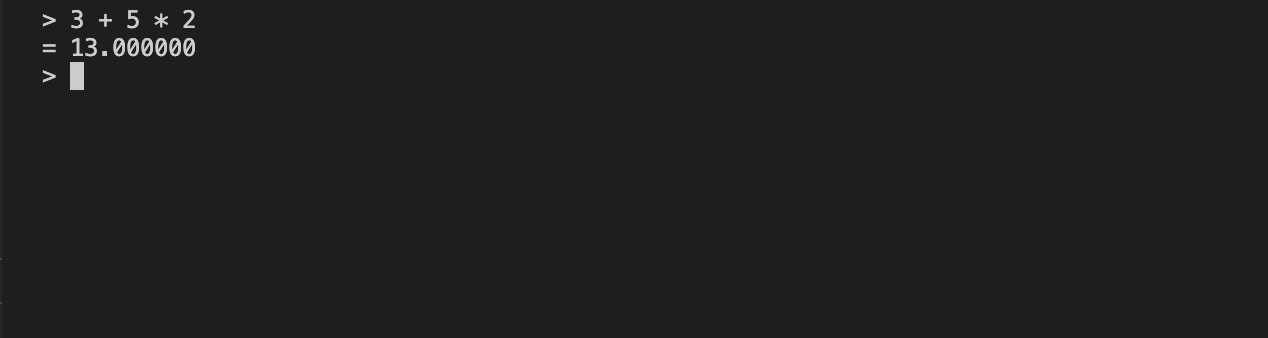
\includegraphics[width=12cm]{naivetest}
	\caption{Демонстрация работы программы}\label{net1}
\end{figure}

\newpage
\section{Сравнение полученных реализаций}

Проведем анализ производительности полученных версий анализатора. В
качестве данных для тестирования возьмем выражения вида 
$\underbrace{2+2+2 \cdots+2}_{n}$
для $n = 1\dots100$ с шагом 1. Для вычисления времени выполнения 
воспользуемся библиотекой \verb"time" Python 3.9.5. Автоматизацию 
обеспечим с помощью библиотеки \verb"subprocess". Получим следующий код:

\inputminted{python}{test.py}

Кроме того, отметим, что в ранее написанные программы были внесены 
некоторые изменения для проведения эксперимента. Ознакомиться с ними
можно в приложении ~\ref{pril-1}.

Ознакомиться с полным исходным кодом программы, осуществляющей
исследование производительности можно в приложении ~\ref{pril-2}.

Для большей наглядности графики интерполированы полиномом с помощью 
функции \verb"polyfit" библиотеки \verb"numpy".

Ознакомиться с полным исходным кодом программы, осуществляющей
анализ полученных результатов можно в приложении ~\ref{pril-3}.

Результаты исследования изображены на рис. ~\ref{net2}:

\begin{figure}[!ht]
	\centering
	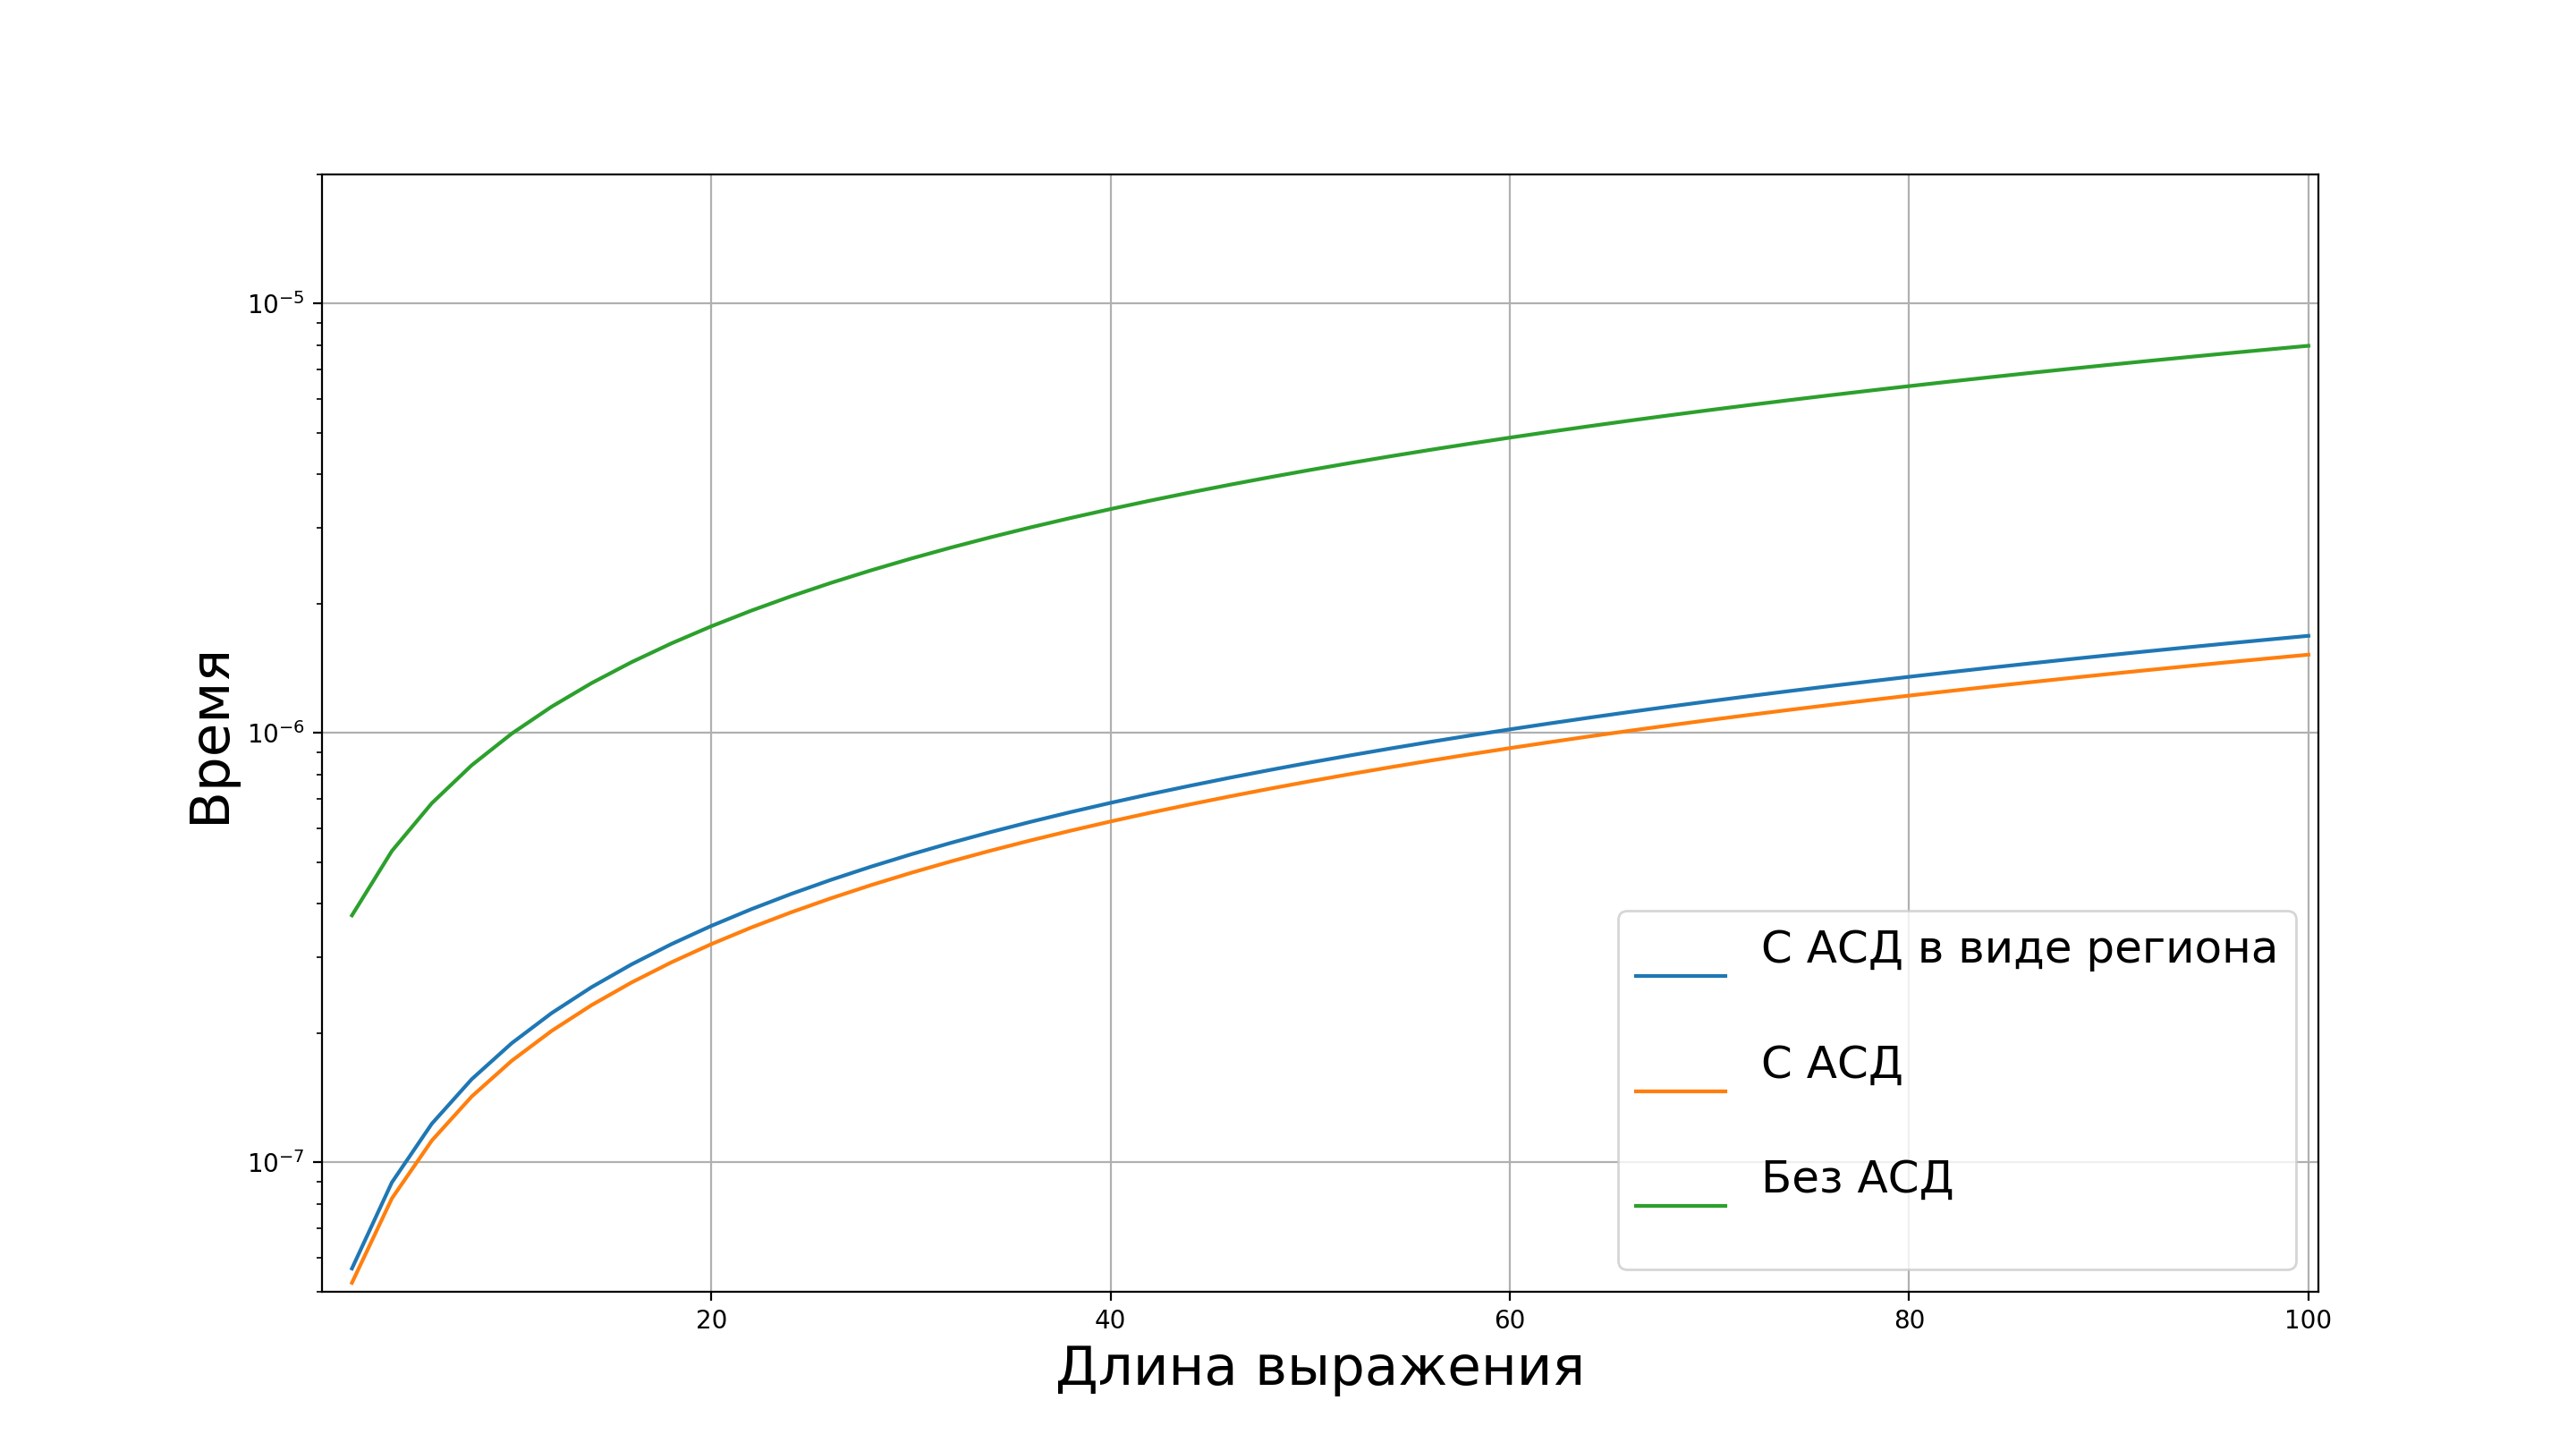
\includegraphics[width=20cm]{benchmark}
	\caption{Демонстрация работы программы}\label{net2}
\end{figure}

Исследование показало, что использование абстрактных синтаксических
деревьев позволяет уменьшить время работы программы более чем в $5$ раз, что
существенно заметно для выражений любой длины.

Также из графиков видно, что в рамках данной работы не удалось добиться 
большей производительности при управлении памятью на основе регионов.
Тем не менее, она все еще может считаться более предпочительной ввиду 
перечисленных ранее преимуществ.

\conclusion

В ходе данной работы:

\begin{enumerate}
    \item Были изучены теоретические основы построения лексических и 
    синтаксических анализаторов.
    \item Проанализированы особенности реализации лексический и 
    синтаксических анализаторов.
    \item Были изучены принципы работы генераторов лексического и 
    синтаксического анализа на примере Flex и GNU Bison.
    \item Были созданы лексический и синтаксический анализаторы для анализа
    математического выражения.
    \item Было изучено понятие абстрактного синтаксического дерева.
    \item Проведен анализ производительности полученных реализаций.
\end{enumerate}

Таким образом, все поставленные в рамках работы задачи выполнены.

Результаты исследования показали, что абстрактные синтаксические 
деревья позволяют добиться увеличения производительности в 5–6 раз.

А это, в свою очередь, позволяет утверждать о том, что концепция 
абстрактных синтаксических деревьев является крайне важной в информатике и
ее приложениях, в частности, при создании синтаксических анализаторов.

\bibliographystyle{gost780uv}
\bibliography{thesis}

\appendix

\section{Flash-носитель с исходным кодом программ, использующихся в работе}\label{pril-1}

\begin{description}
\item[Папка] \verb"src" содержит оригинальный исходный код программы:
\begin{description}
    \item[Папка] \verb"naive" "--- реализация без АСД
    \item[Папка] \verb"naiveast" "--- реализация с АСД
    \item[Папка] \verb"arena" "--- реализация с АСД на основе региона
\end{description}
\item[Папка] \verb"extsrc" содержит измененный исходный код, необходимый для исследования производительности:
\begin{description}
    \item[Папка] \verb"naive" "--- реализация без АСД
    \item[Папка] \verb"naiveast" "--- реализация с АСД
    \item[Папка] \verb"arena" "--- реализация с АСД на основе региона
\end{description}
\end{description}

\section{Исходный код программы на Python, осуществляющей исследование производительности полученных реализаций}\label{pril-2}

\inputminted[]{python}{test.py}

\section{Исходный код программы на Python, осуществляющей анализ полученных результатов}\label{pril-3}

\begin{minted}{python}
import subprocess as sb
from time import time
import matplotlib.pyplot as plt
import sys
import numpy as np

legend = []
for index in range(1, len(sys.argv)):
    file_name = sys.argv[index]
    f = open(file_name, "r")
    try:
        parser_type = f.readline()
    except StopIteration:
        parser_type = "Undefined parser"
    legend.append(parser_type)
    
    x_axis = []
    y_axis = []
    for line in f:
        try:
            w, h = [float(x) for x in next(f).split()] 
        except StopIteration:
            break
        x_axis.append(w)
        y_axis.append(h)
    plt.xlabel("Длина выражения", size = 22)
    plt.ylabel("Время", size = 22)
    p = np.polyfit(x_axis, y_axis, 1)
    for i in range(len(x_axis)):
       y_axis[i] = p[0] * x_axis[i] + p[1]
    
    plt.plot(x_axis, y_axis)
plt.xlim(0.5, 100.5)
plt.ylim(5e-8, 2e-5)
plt.rcParams.update({'font.size': 18})
#plt.yscale("log")
plt.grid(True) 
plt.legend(legend, loc="lower right")
plt.show()
\end{minted}
\end{document}